
「量子コンピュータや量子プログラミングに興味はあるが、何から手を付けたら良いか分からない」という方は多いのではないでしょうか。
量子を使うと何が変わるのか、0と1を同時に表現すると何が便利ですごいのか。これらは量子情報の研究者や量子コンピュータを研究開発する企業、報道関係者など、量子コンピュータに関わる人が常に苦心しながら様々な表現を試みています。

量子コンピュータの開発企業でもあるIBMでは、少しでも量子コンピュータについて理解してもらうための試みとして、スマートフォン向けゲームを提供しています。このコピー本では、このゲームの遊び方、特に、独特な量子状態の表現方法について紹介します。

\section*{Hello Quantum}
\addcontentsline{toc}{section}{Hello Quantum}
\label{sec:1-1}

Hello Quantumと名付けられたこのゲームは、2つの量子ビットを操作して目的の状態を目指すパズルです。X・Z・H・CZといった基本的な量子ゲートが提供されており、プレイヤーはこれらを順次作用させてパズルを解くことができます。
ゲームはステージ制になっており、最善手の手数が目標として示されています。レベルが上がるほど利用できる量子ゲートの種類や必要な手数が増えるようになっています。

\begin{reviewimage}
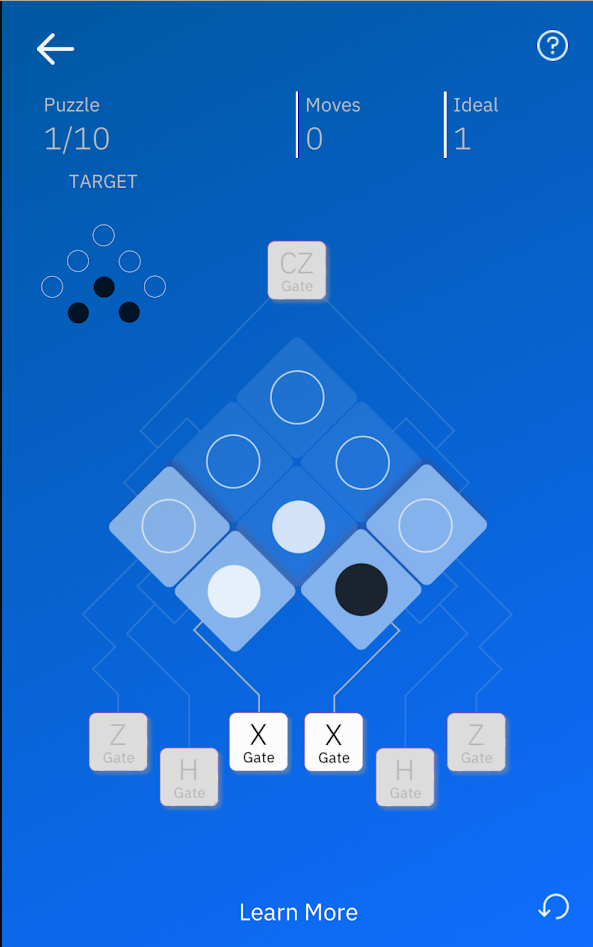
\includegraphics[width=0.2\maxwidth]{./images/image0.png}
\caption{プレイ画面。Google Playアプリページより(iOS版もあります)}
\label{image:01:image0}
\end{reviewimage}

\section*{画面の見方}
\addcontentsline{toc}{section}{画面の見方}
\label{sec:1-2}

画面下の2つがそれぞれ量子ビットの状態を示します。以下の図では右下が第一量子ビット、左下が第二量子ビットです。

\begin{reviewimage}
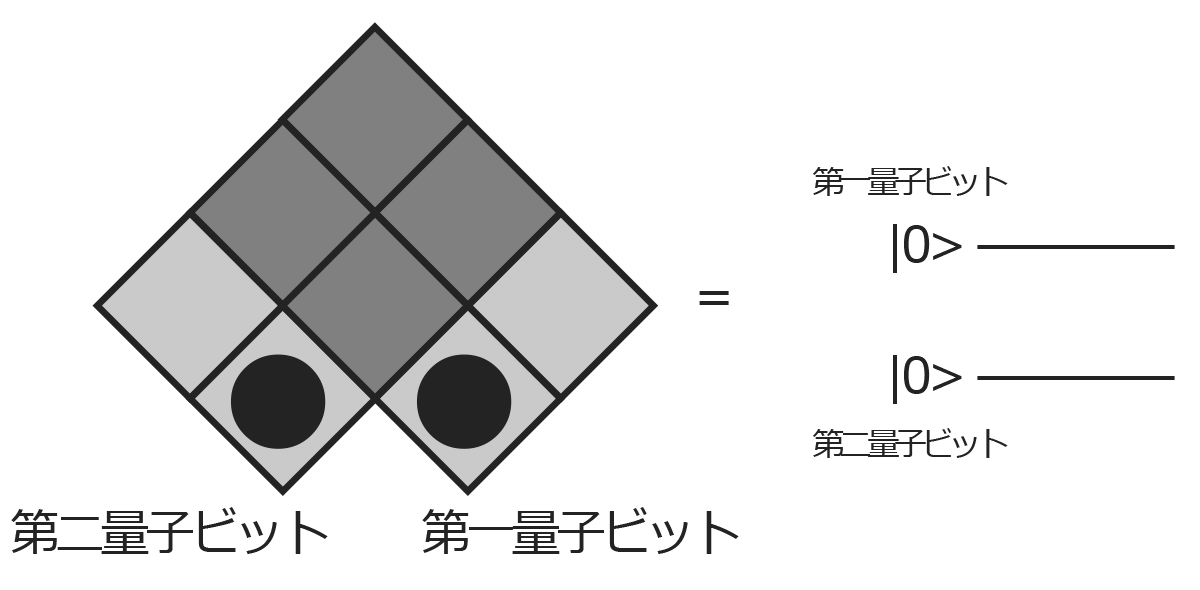
\includegraphics[width=0.8\maxwidth]{./images/image1.png}
\caption{基本の量子状態}
\label{image:01:image1}
\end{reviewimage}

\section*{量子ビット}
\addcontentsline{toc}{section}{量子ビット}
\label{sec:1-3}

1つの量子ビットは2つのグリッドで構成され、グリッドそれぞれには、黒丸・白丸・輪郭だけの丸のいずれかが入っています。

2つのグリッドはその量子ビットに対してどのような基底で測定するか、グリッド内の丸は測定結果としてどのような結果が得られるかを表しています。

黒丸はその基底における基底状態を、白丸は励起状態が得られることを示します。輪郭だけの丸は、その基底での測定結果はランダムに得られることを示しています。
基底における基底状態、という言い回しはわかりづらいのですが、測定に用いる基底は直交する状態ベクトルのペアであり、\textbar{}0\textgreater{}と\textbar{}1\textgreater{}のペア(計算基底と呼ばれるもの)や\textbar{}+\textgreater{}と\textbar{}{-}\textgreater{}のペアです。
基底状態とは、普通のコンピュータのビットで言えば電圧が低い状態、励起状態とは電圧が高い状態に相当します。

\begin{reviewimage}
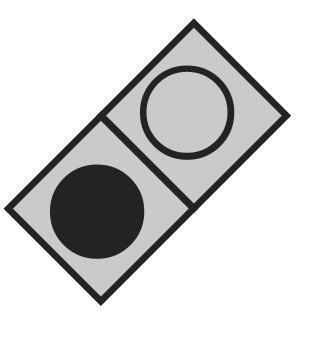
\includegraphics[width=0.3\maxwidth]{./images/image2s.png}
\caption{単一量子ビットの例}
\label{image:01:image2s}
\end{reviewimage}

黒丸は計算基底における基底状態\textbar{}0\textgreater{}を、白丸は励起状態\textbar{}1\textgreater{}を、輪郭はランダムで不定であることを示します。
同様に、上側の格子にも丸が入っています。こちらは\textbar{}+\textgreater{}\textbar{}{-}\textgreater{}基底における状態を表しており、黒丸は\textbar{}+\textgreater{}\textbar{}{-}\textgreater{}基底における基底状態(つまり\textbar{}+\textgreater{})を、白丸は励起状態\textbar{}{-}\textgreater{}を得られることを示します。

\begin{reviewimage}
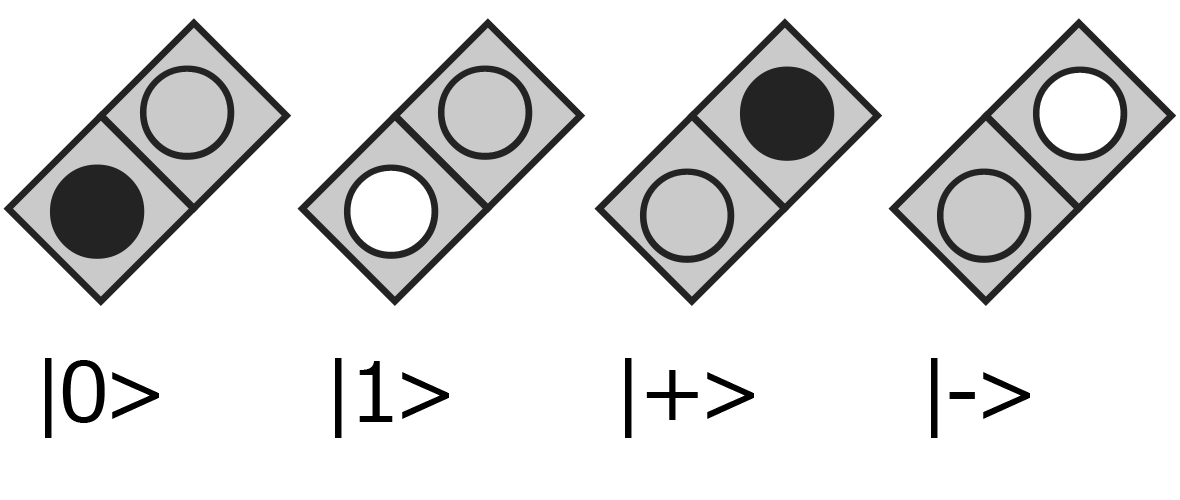
\includegraphics[width=0.75\maxwidth]{./images/image2.png}
\caption{各量子状態}
\label{image:01:image2}
\end{reviewimage}

Hello Quantumで操作できる量子ビットは2つあるので、それぞれがとりうる状態の数は組み合わせの数だけあります。これを表現しているのが中央の4つの格子です。
それぞれ量子ビットから、グリッドに沿って中央向けてに伸ばした時、中央の4つのグリッドのどれかで交差します。
ここに2つの量子ビットの状態に応じて丸を書き込みます。
つまり、グリッドのどこに丸が書きこまれているか見れば、2つの量子ビットを測定したとき、どのような測定結果が得られるか知ることができます。

\begin{reviewimage}
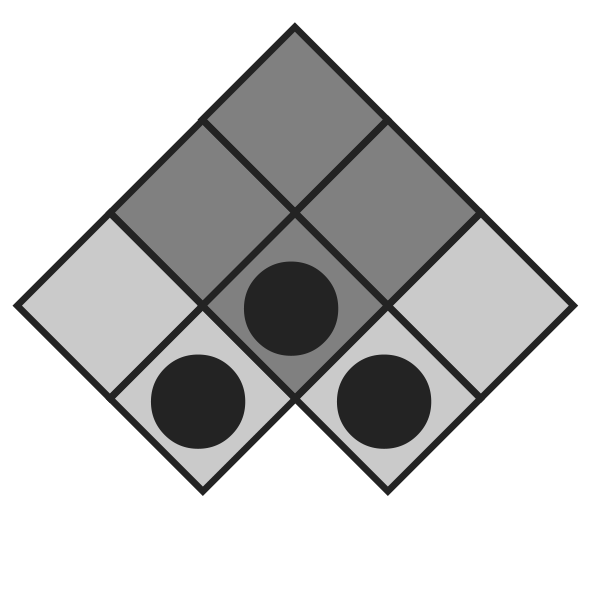
\includegraphics[width=0.5\maxwidth]{./images/image4.png}
\caption{中央のグリッドの例}
\label{image:01:image4}
\end{reviewimage}

どのグリッドに黒丸が書きこまれるかは、以下の法則にまとめられます。

\begin{table}%%statelist
\reviewtablecaption{量子ビットと中央グリッドの黒丸の対応}
\label{table:01:statelist}
\begin{reviewtable}{|l|l|l|}
\hline
\reviewth{グリッド位置} & \reviewth{条件} & \reviewth{状態ベクトル} \\  \hline
トップ & Z・Z基底測定で2量子ビットの測定物理量は一致 & \textbar{}++\textgreater{} or \textbar{}{-}{-}\textgreater{} \\  \hline
ボトム & X・X基底測定で2量子ビットの測定物理量は一致 & \textbar{}00\textgreater{} or \textbar{}11\textgreater{} \\  \hline
レフト & X・Z基底測定で2量子ビットの測定物理量は一致 & \textbar{}0+\textgreater{} or \textbar{}1{-}\textgreater{} \\  \hline
ライト & Z・X基底測定で2量子ビットの測定物理量は一致 & \textbar{}+0\textgreater{} or \textbar{}{-}1\textgreater{} \\  \hline
\end{reviewtable}
\end{table}

白丸が書き込まれた場合、一致ではなく不一致することを示します。例えばグリッドのトップに白丸があれば、それは\textbar{}+{-}\textgreater{} or \textbar{}+{-}\textgreater{}状態を表します。

\begin{table}%%statelist
\reviewtablecaption{量子ビットと中央グリッドの白丸の対応}
\label{table:01:statelist}
\begin{reviewtable}{|l|l|l|}
\hline
\reviewth{グリッド位置} & \reviewth{条件} & \reviewth{状態ベクトル} \\  \hline
トップ & Z・Z基底測定で2量子ビットの測定物理量は不一致 & \textbar{}+{-}\textgreater{} or \textbar{}{-}+\textgreater{} \\  \hline
ボトム & X・X基底測定で2量子ビットの測定物理量は不一致 & \textbar{}10\textgreater{} or \textbar{}01\textgreater{} \\  \hline
レフト & X・Z基底測定で2量子ビットの測定物理量は不一致 & \textbar{}0{-}\textgreater{} or \textbar{}1+\textgreater{} \\  \hline
ライト & Z・X基底測定で2量子ビットの測定物理量は不一致 & \textbar{}+1\textgreater{} or \textbar{}{-}0\textgreater{} \\  \hline
\end{reviewtable}
\end{table}

\section*{基本的な量子ゲート}
\addcontentsline{toc}{section}{基本的な量子ゲート}
\label{sec:1-4}

Hello QuantumではX・Z・Hの量子ゲートを作用させることができます。これは実際にアプリでゲートを作用させて眺めたほうが分かりやすいのではないでしょうか。

注意点として、Hello Quantumでは負の係数は表現されていません。つまり、\textbar{}1\textgreater{} にZを作用させると{-}\textbar{}1\textgreater{}になりますが、この{-}は可視化されないということです。

\begin{reviewimage}
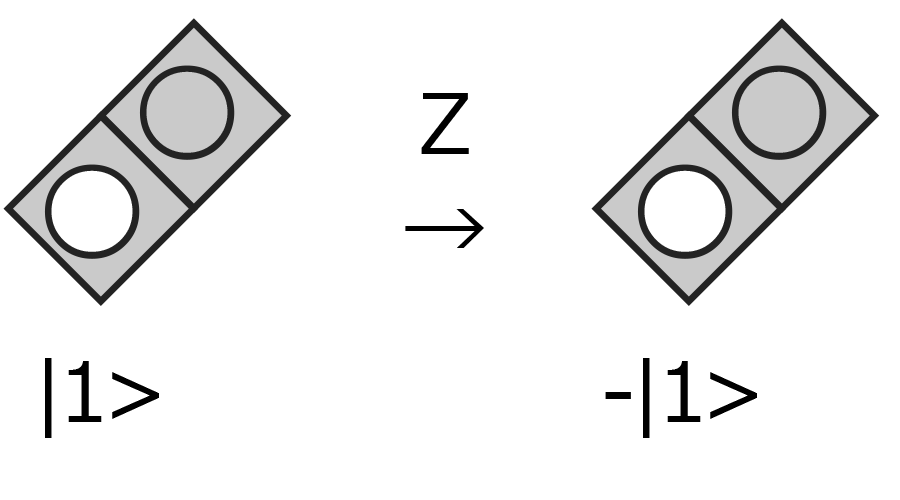
\includegraphics[width=0.75\maxwidth]{./images/image5.png}
\caption{係数は表現されない}
\label{image:01:image5}
\end{reviewimage}

これはHello Quantum作者の一人James Woottonも言及しており、\footnote{https://medium.com/qiskit/hello{-}quantum{-}2c1c00fe830c}この表現には1量子ビットあたりグリッドが3つ必要になり、
2量子ビットを正確に表すためには中央のグリッドが9つ、合計で15のグリッドが必要になってしまうとされています。

\section*{CZを用いたセパラブルでない量子状態}
\addcontentsline{toc}{section}{CZを用いたセパラブルでない量子状態}
\label{sec:1-5}

Hello QuantumのLevel.3からは、CZゲート(制御Zゲート)を利用できるようになります。これは2量子ビットに作用するので、他の量子ゲートと組み合わせることで重ね合わせ状態を作れるようになります。
これもアプリ上で作用させるのが直観的で分かりやすいですが、CZを作用させると、各量子ビットと中央のグリッドの接線を軸に丸の位置を交換します。

例として、\textbar{}{-}{-}\textgreater{}に対してCZを作用させることを考えます。

\begin{reviewimage}
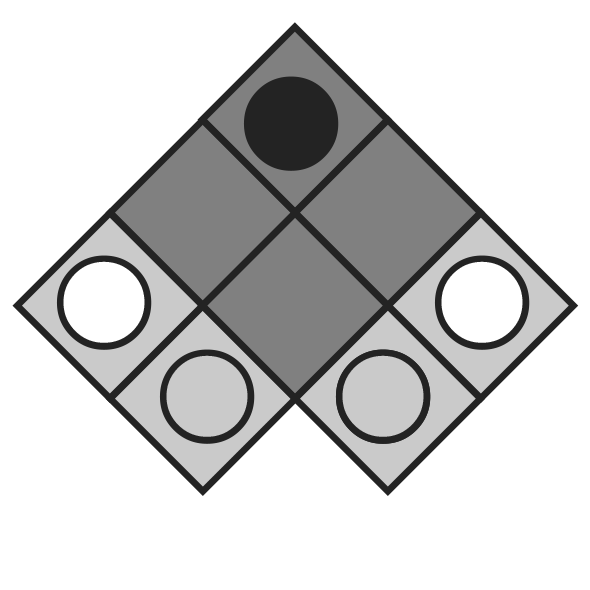
\includegraphics[width=0.5\maxwidth]{./images/image6.png}
\caption{\textbar{}{-}{-}\textgreater{}}
\label{image:01:image6}
\end{reviewimage}

これにCZを作用させると、

\begin{reviewimage}
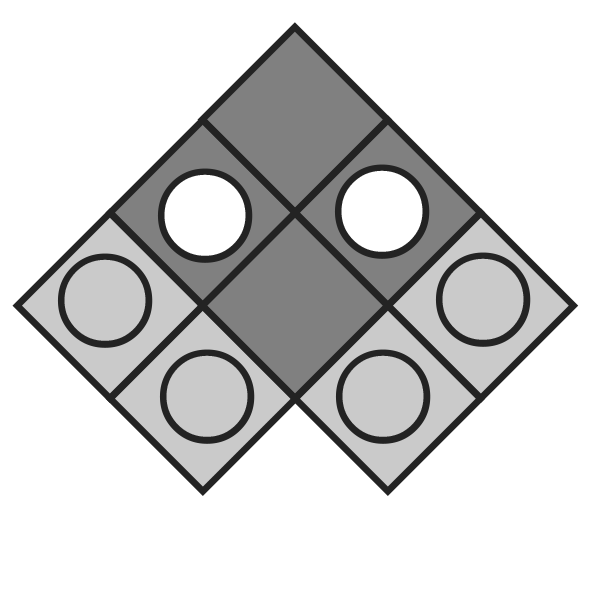
\includegraphics[width=0.5\maxwidth]{./images/image7.png}
\caption{\textbar{}{-}{-}\textgreater{} {-} \textbar{}11\textgreater{}}
\label{image:01:image7}
\end{reviewimage}

\textbar{}{-}{-}\textgreater{} {-} \textbar{}11\textgreater{}になります。\textbar{}{-}{-}\textgreater{} {-} \textbar{}11\textgreater{}は重ね合わせ状態なので、各量子ビットの状態は一意に定まっていません。よって、左右下のグリッドはすべて輪郭だけの丸になります。

また、\textbar{}{-}{-}\textgreater{} {-} \textbar{}11\textgreater{}を状態ベクトルをもとに変形すれば、\textbar{}0{-}\textgreater{} {-} \textbar{}1+\textgreater{}や\textbar{}{-}0\textgreater{} {-} \textbar{}+1\textgreater{}に置き換えることができます。

\begin{equation*}
    \begin{split}
		\left| -- \right> - \left| 11 \right> =& \frac{1}{2} \left( \left| 00 \right> - \left| 01 \right> - \left| 10 \right> + \left| 11 \right> \right) + \left| 11 \right> \\
		&= \frac{1}{2} \left( \left| 00 \right> - \left| 01 \right> - \left| 10 \right> - \left| 11 \right> \right) \\
		&= \left| 0- \right> - \left| 1+ \right> = \left| -0 \right> - \left| +1 \right>
    \end{split}
\end{equation*}

\textbar{}0{-}\textgreater{} {-} \textbar{}1+\textgreater{}ということは、先の表で言えばグリッドのレフトに白丸があるということです。同様に、\textbar{}{-}0\textgreater{} {-} \textbar{}+1\textgreater{}はライトに白丸があります。
グリッドのレフトとライトに白丸があることは、\reviewimageref{1.8}{image:01:image7}のグリッドの状態と同じです。

\section*{補足}
\addcontentsline{toc}{section}{補足}
\label{sec:1-6}

Hello Quantumについて良く分かっていない挙動として、\textbar{}10\textgreater{}{-}\textbar{}01\textgreater{}に対してCZを作用させると、本来作用しないはずのパウリZが作用し、グリッドトップの丸が黒に反転します。
これはバグなのか、著者の理解が足りていないためなのかは調査中です。
